\chapter{From MDPs to Reinforcement Learning}
\label{chapter3}

\vspace{0.5cm}

\noindent As said before, when we have both the reward function $\mathcal{R}$ and the transition model $\mathcal{P}$ we can solve the MDP by means of dynamic programming.

Truth to be told, for most cases we cannot precisely predict neither $\mathcal{R}$ nor $\mathcal{P}$ and we have to approximate, explore and estimate functions and states in order to converge to the optimal solution (the optimal policy).

Reinforcement Learning in fact, is a technique to handle Markov Decision Processes in an environment we don't fully know.

\section{Value Function and the Bellman equation}
We spoke before about \textit{optimal policy} but we never defined it. The optimal policy, is the one that maximizes our long term expected reward, that is:
\begin{equation}
    \pi^\star = arg\,max_\pi \ \mathbb{E} \Big[ \sum_t \gamma^t \mathcal{R}(s_t) \ \vert \ \pi \Big]
\end{equation}
\noindent
We can see in this function, that the initial state is not defined (it's random), and that the optimal policy must be optimal starting from any state.

We can actually define also the \textbf{value function} that gives the expected long term reward following a policy starting from a state $s$:
\begin{equation}
    \mathbb{V}^\pi(s) = \mathbb{E} \Big[ \sum_t \gamma^t \mathcal{R}(s_t) \ \vert \ \pi, \ s_0 = s \Big]
\end{equation}
This function helps us to define in a better way the optimal policy:
\begin{equation} \label{eq:bellman-value}
    \pi^\star = arg\,max_a \ \sum_{s'} \mathbb{P}(s_{t+1} = \mathnormal{s'} \vert s_t = \mathnormal{s}, a_t = \mathnormal{a}) \ \mathbb{V}(s')
\end{equation}
This equation says that the optimal policy is the one that, for every state, returns the action that maximizes my expected value function and this allows us to write the value function in a much more famous form known as \textbf{Bellman Equation}:
\begin{equation}
    \mathbb{V}^\pi(s) = \mathcal{R}(s) +  \gamma\sum_{s'} \mathbb{P}(s_{t+1} = \mathnormal{s'} \vert s_t = \mathnormal{s}, a_t = \mathnormal{a}) \ \mathbb{V}(s')
\end{equation}
This equation has two terms and says that the expected sum of discounted return is equal to the sum of two terms: the initial, or immediate, reward received immediately simply for starting in state $s$, and a discounted sum of the future expected rewards (rewards after the first step) and can be rewritten as \begin{equation}
    \mathbb{V}^{\pi^\star}(s) = \mathcal{R}(s) +  \gamma\,max_a\sum_{s'} \mathbb{P}(s_{t+1} = \mathnormal{s'} \vert s_t = \mathnormal{s}, a_t = \mathnormal{a}) \ \mathbb{V}(s')
\end{equation}
to describe the optimal value function $\mathbb{V}^\star$.

\section{Action-value function}
\begin{comment}
\begin{figure}[ht]
    \centering
    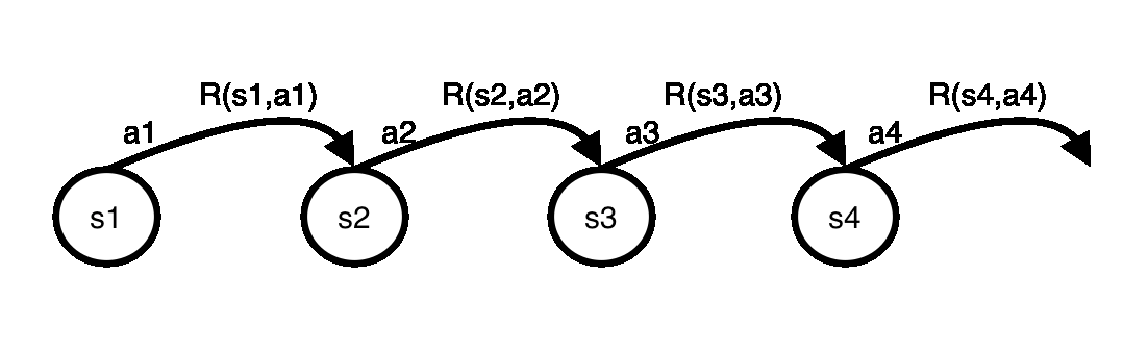
\includegraphics[width=1\textwidth]{./pictures/bellman.eps}
    \caption{A representation of the Bellman equation.}
    \label{fig:bellman}
\end{figure}
\end{comment}
\begin{figure} [ht]    
    \tikzstyle{squarenode} = [circle, draw, minimum size=5mm]
        
    \centering
    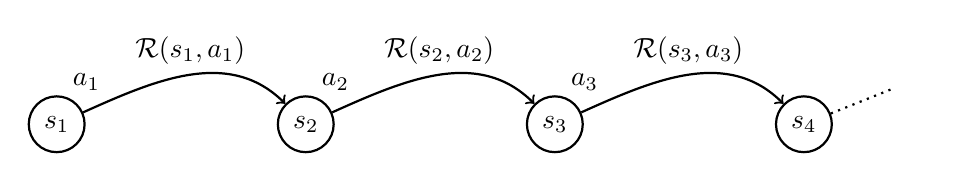
\begin{tikzpicture}[align = center, node distance = 9em, auto, thick]
        \node [squarenode] (s1) {$s_1$};
        \node [squarenode, right of=s1] (s2) {$s_2$};
        \node [squarenode, right of=s2] (s3) {$s_3$};
        \node [squarenode, right of=s3] (s4) {$s_4$};
        \node[squarenode,draw=none, right of=s4, xshift=-5em, yshift=1.6em] (s5) {};

        \draw [->] (s1) edge [out=90 in=90] node[right, above] {$\mathcal{R}(s_1, a_1)$} node[very near start] {$a_1$} (s2);
        \draw [->] (s2) edge [out=90 in=90] node[right, above] {$\mathcal{R}(s_2, a_2)$} node[very near start] {$a_2$}  (s3);
        \draw [->] (s3) edge [out=90 in=90] node[right, above] {$\mathcal{R}(s_3, a_3)$} node[very near start] {$a_3$}  (s4);
        \draw (s4) edge [dotted] node {}  (s5);

    \end{tikzpicture}
    \caption{A representation of Bellman equation.}
    \label{fig:bellman}
\end{figure}
The Bellman equation is fundamental and is a necessary condition for optimality. Visually, our system goes like the one depicted in figure \ref{fig:bellman} and the Bellman Equation~(\ref{eq:bellman-value}) describes this system immediately after state $s_1$, before taking action $a_1$, so when we talk about \textit{value} we talk about a state and eventually we will get into another state that can also be represented with another value function. This is why the Bellman equation can be depicted in a recursive way.

The purpose of explaining the Bellman equation graphically is to show that, as the value function shows the infinite recursion of the system starting from state $s$, we can actually represent this recursion, starting immediately after the action is taken.

This equation is called \textbf{action-value function} and is defined in two ways. The first one in the Bellman equation form:
\begin{equation}
    \mathbb{Q}^\pi(s, a) = \mathcal{R}(s, a) +  \gamma\sum_{s'} \mathbb{P}(s_{t+1} = \mathnormal{s'} \vert s_t = \mathnormal{s}, a_t = \mathnormal{a}) \ \,max_a\mathbb{Q}(s', a')
\end{equation}
and the second one in the expectation form:
\begin{equation}
    \mathbb{Q}^\pi(s, a) = \mathbb{E} \Big[ \sum_t \gamma^t \mathcal{R}(s_t) \ \vert \ \pi, \ s_0 = s, \ a_0 = a \Big]
\end{equation}
This equations can be explained as we are in state $s$, we take action $a$, we get the first reward that is the first term, and then we go on with the summation.

The optimal value and action value functions are related in the following way.
\begin{align*}
    \mathbb{V}^\star(s) &= \,max_a\mathbb{Q}^\star(s, a) \\
    \mathbb{Q}^\star(s, a) &= \mathcal{R}(s, a) +  \gamma\sum_{s'} \mathbb{P}(s_{t+1} = \mathnormal{s'} \vert s_t = \mathnormal{s}, a_t = \mathnormal{a}) \ \mathbb{V}^\star(s')
\end{align*}
One way of thinking about this is: we always go further in the cycle. For the value function, we need the best possible action and the state-action function has already taken an action, so I just get the max state-action function. Same way for the second function, state-action function starts after the action is taken, so I sum the reward and I continue at the landing state so with the value function.

Someone may ask themselves \textit{why are we bothering of creating this action-value function when we already have the value function?} \\
Well, the \textit{action-value function} is key in reinforcement learning as it allows to take expectations of $\mathbb{Q}^\pi(s,a)$ without knowing the transition function or the reward function.

\section{Algorithms}
Now that we have defined two important functions, we can describe a reinforcement learning algorithm.

\subsection{Introduction}
\begin{figure} [ht]
    \tikzstyle{block} = [rectangle, draw, 
        text width=8em, text centered, rounded corners, minimum height=4em]
        
    \tikzstyle{line} = [draw, -latex]
    \centering
    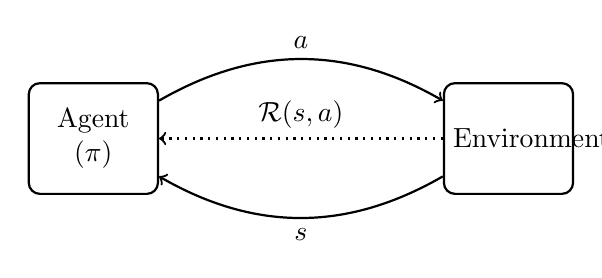
\begin{tikzpicture}[align = center, node distance = 15em, auto, thick]
        \node [block] (Agent) {Agent ($\pi$)};
        \node [block, right of=Agent] (Environment) {Environment};
        \draw [->] (Agent) edge [bend left]  node {$a$} (Environment);
        \draw [->] (Environment) edge [bend left] node {$s$}  (Agent);
        \draw [->] (Environment) edge [dotted] node [above] {$\mathcal{R}(s,a)$} (Agent);
    \end{tikzpicture}
    \caption{The concept of reinforcement learning.}
    \label{fig:rldiagram}
\end{figure}
\noindent
To understand better reinforcement learning, it's better to see Figure~\ref{fig:rldiagram}. The environment reveals to the agent in forms of states and the agent replies with actions and the environment sends back a reward. All the computation or, in a more reinforcement learning way, the \textit{thinking}, is done in the agent \textit{mind} through the policy. \\
An important concept is that the information regarding the environment is only available through this interaction, meaning that the environment is not available in the agent's brain (the policy), but the agent is \textit{experiencing} the environment only by interacting with it.

\subsection{Different families of algorithms}
We can think of a RL algorithm as a method that, given a sequence of action-state-reward triplets, is able to find an optimal policy $\pi$ as depicted in Figure~\ref{fig:rlalg-general}.
\begin{figure} [ht]
    \tikzstyle{block} = [rectangle, draw, 
        text width=8em, text centered, rounded corners, minimum height=4em]
    \tikzstyle{txtblock} = [rectangle, 
        text width=8em, text centered, rounded corners, minimum height=4em]
        
    \tikzstyle{line} = [draw, -latex]
    \centering
    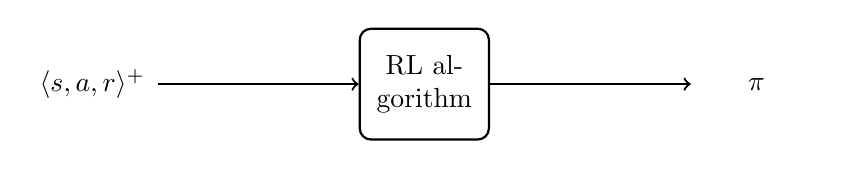
\begin{tikzpicture}[align = center, node distance = 15em, auto, thick]
        \node [txtblock] (sequence) {$\langle s, a, r \rangle^+$};
        \node [block, right of=sequence, xshift=-3em] (algorithm) {RL algorithm};
        \node [txtblock, right of=algorithm, xshift=-3em] (policy) {$\pi$};
        \draw [->] (sequence) edge  node {} (algorithm);
        \draw [->] (algorithm) edge node {}  (policy);
    \end{tikzpicture}
    \caption{Reinforcement learning algorithm}
    \label{fig:rlalg-general}
\end{figure}
The RL algorithm block can be split in different ways according to the way the policy is learned. We can divide algorithms in three main families.

\subsubsection{Model-based algorithms}
\begin{figure} [ht]
    \tikzstyle{block} = [rectangle, draw, 
        text width=4em, text centered, rounded corners, minimum height=4em]
    \tikzstyle{txtblock} = [rectangle, 
        text width=4em, text centered, rounded corners, minimum height=4em]
        
    \tikzstyle{line} = [draw, -latex]
    \centering
    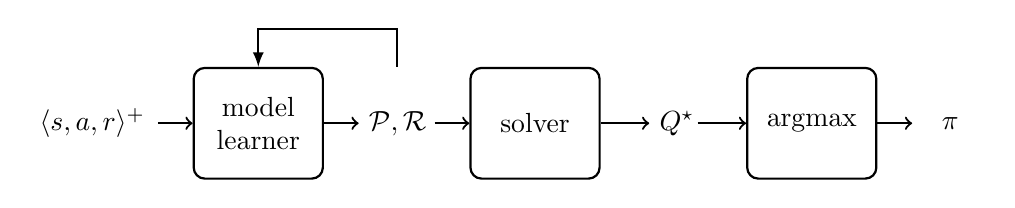
\begin{tikzpicture}[align = center, node distance = 15em, auto, thick]
        \node [txtblock] (sequence) {$\langle s, a, r \rangle^+$};
        \node [block, right of=sequence, xshift=-9em] (model-learner) {model learner};
        \node [txtblock, text width=2em, right of=model-learner, xshift=-10em] (p-r) {$\mathcal{P}, \mathcal{R}$};
        \node [block, right of=p-r, xshift=-10em] (solver) {solver};
        \node [txtblock, text width=1em, right of=solver, xshift=-10em] (action-value) {$\mathbb{Q}^\star$};
        \node [block, right of=action-value, xshift=-10em] (argmax) {argmax};
        \node [txtblock, text width=2em, right of=argmax, xshift=-10em] (policy) {$\pi$};
        \draw [->] (sequence) edge  node {} (model-learner);
        \draw [->] (model-learner) edge node {}  (p-r);
        \draw [->] (p-r) edge node {}  (solver);
        \draw [->] (solver) edge node {}  (action-value);
        \draw [->] (action-value) edge node {}  (argmax);
        \draw [->] (argmax) edge node {}  (policy);
        \path [line] (p-r) |-++ (0cm, 1.2cm) -| (model-learner);

    \end{tikzpicture}
    \caption{A model-based algorithm}
    \label{fig:model-based}
\end{figure}
\noindent
A \textbf{model-based} algorithm takes the action-state-reward triples and sends them to a \textit{model learner} which learns the transition probability function $\mathcal{P}$ and the reward function $\mathcal{R}$. Once learned, a solver can compute an optimal action-value function. Once you have an optimal action-value function, for each state you just get the argmax to get the best action, and that's the policy.
The reason we have an arrow going back in the model learner is that the transition probability and the reward functions are initially estimated and are continuously updated with previous values of the functions.

\subsubsection{Value-function based algorithms}
\begin{figure} [ht]
    \tikzstyle{block} = [rectangle, draw, 
        text width=4em, text centered, rounded corners, minimum height=4em]
    \tikzstyle{txtblock} = [rectangle, 
        text width=4em, text centered, rounded corners, minimum height=4em]
        
    \tikzstyle{line} = [draw, -latex]
    \centering
    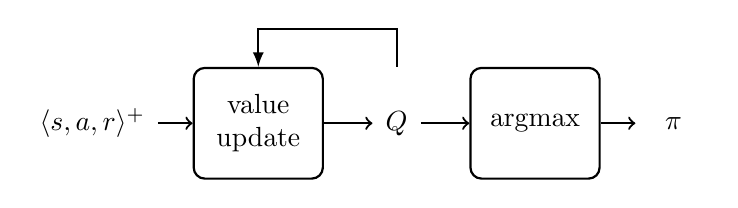
\begin{tikzpicture}[align = center, node distance = 15em, auto, thick]
        \node [txtblock] (sequence) {$\langle s, a, r \rangle^+$};
        \node [block, right of=sequence, xshift=-9em] (value-update) {value update};
        \node [txtblock, text width=1em, right of=value-update, xshift=-10em] (action-value) {$\mathbb{Q}$};
        \node [block, right of=action-value, xshift=-10em] (argmax) {argmax};
        \node [txtblock, text width=2em, right of=argmax, xshift=-10em] (policy) {$\pi$};
        \draw [->] (sequence) edge  node {} (value-update);
        \draw [->] (value-update) edge node {}  (action-value);
        \draw [->] (action-value) edge node {}  (argmax);
        \draw [->] (argmax) edge node {}  (policy);
        \path [line] (action-value) |-++ (0cm, 1.2cm) -| (value-update);

    \end{tikzpicture}
    \caption{A value-function based algorithm}
    \label{fig:value-function-based}
\end{figure}
\noindent
The \textbf{value-function} based algorithms are almost the same as the previous family of algorithms except that, as we can see from figure~\ref{fig:value-function-based}, one block is missing. The main difference is that this family of algorithms tries to learn a policy without explicitly learning the model or better, the policy is learned without the assumption of knowing the model, whereas in the first family, to learn the policy, the model \textit{must} be learned (the two functions that define a model are the transition probability function and the reward function).
This family of algorithm is in fact also called \textbf{model-free algorithms}.

In this family, the state-action function is directly estimated from the sequence of tuples from the environment and previous values of $\mathcal{Q}$. The $\mathcal{Q}$ doesn't have a $\star$ since it's just an estimation and it's not an optimal value but, with continuous iterations, it is proven that it will reach an optimal value.

\subsubsection{Policy search algorithms}
\begin{figure} [ht]
    \tikzstyle{block} = [rectangle, draw, 
        text width=4em, text centered, rounded corners, minimum height=4em]
    \tikzstyle{txtblock} = [rectangle, 
        text width=4em, text centered, rounded corners, minimum height=4em]
        
    \tikzstyle{line} = [draw, -latex]
    \centering
    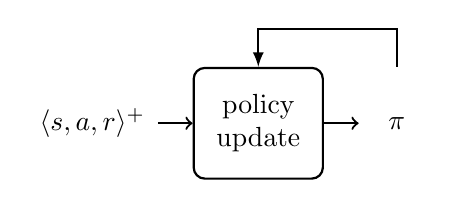
\begin{tikzpicture}[align = center, node distance = 15em, auto, thick]
        \node [txtblock] (sequence) {$\langle s, a, r \rangle^+$};
        \node [block, right of=sequence, xshift=-9em] (policy-update) {policy update};
        \node [txtblock, text width=2em, right of=policy-update, xshift=-10em] (policy) {$\pi$};
        \draw [->] (sequence) edge  node {} (policy-update);
        \draw [->] (policy-update) edge node {}  (policy);
        \path [line] (policy) |-++ (0cm, 1.2cm) -| (policy-update);
    \end{tikzpicture}
    \caption{A policy search algorithm}
    \label{fig:policy-search}
\end{figure}
\noindent
The third family of algorithms updates directly the policy by feeding it back to the policy update that modifies it based on the sequence that it receives. This algorithm is much more direct, but the learning problem is much more difficult because the feedback you get from the policy usually is not that useful to update it. For example, in a game, knowing that an action moves you forward isn't sufficient to know when to use it.
\newline
\newline
As depicted in figures~\ref{fig:model-based}, \ref{fig:value-function-based} and \ref{fig:policy-search}, we can see that the three algorithms are getting simpler as going down, meaning that the policy learning is more direct but in the opposite way, going up, the algorithms become more supervised. Most of the time of this semester project has been spent in model-free value-based algorithms that provide a good balance between learning techniques and learning difficulties.

\subsection{Off-policy and on-policy algorithms}
A further distinction between algorithms can be made through another aspect, if they are \textit{off-policy} or \textit{on-policy}.

\begin{itemize}
    \item \textbf{off-policy} algorithms are those algorithms that learn about the greedy strategy (policy), while following a different policy that allows a better exploration of the state space;
    \item \textbf{on-policy} algorithms are those algorithms that estimate functions according to the current policy.
\end{itemize}

An on-policy algorithm is influenced by the exploration policy and can get stuck in a local maximum whereas an off-policy algorithm is independent from the exploration policy and reaches the global optimum. \\
Algorithmically, an on-policy algorithm updates its $\mathcal{Q}$-values using the $\mathcal{Q}$-value of the next state $s'$ and the current policy's action $a'$ so it estimates the return for state-action pairs assuming the \textit{current policy} continues to be followed. An off-policy algorithm updates its $\mathcal{Q}$-values using the $\mathcal{Q}$-value of the next state $s'$ and the greedy action $a'$ so it estimates the return for state-action pairs assuming a \textit{greedy policy} was followed despite the fact that it is not following a greedy policy. \\
This distinction disappears when the followed policy is a greedy policy but an agent that works like this wouldn't be as good since it would never explore the space of solutions.

%policy based
%value based
%model based
%model free

%off-on policy
%actor algorithm
%critic algorithms
%actor critic algorithms

\subsection{Deep Q-Network}

\textbf{Deep Q-Network}, or \textbf{DQN}, is the first popular reinforcement learning algorithm, proposed by DeepMind in 2013~\cite{pongpixels}.

It's an updated version of the Q-learning algorithm first proposed by Watkins in 1992~\cite{Watkins1992} and uses deep learning to estimate the action-value function. The Q-network is the neural network function approximator with parameters $\theta$.

Since it approximates and updates the action-value function, DQN is a \textit{model-free}, \textit{value-function based} algorithm: it solves the reinforcement learning task directly using samples from the emulator, without explicitly constructing an estimate of the model.

The two main characteristics regarding this algorithm are how it approximates the action-value function and the \textbf{experience replay}'s concept.
\subsubsection{Deep Reinforcement Learning}
Deep reinforcement learning can be defined as the connection between reinforcement Learning and neural networks, started in the late 90s~\cite{Tesauro1994} but with DQN it started to get exciting achievements and visibility. The deep reinforcement learning part is in the approximation of the action-value function with a convolutional neural network with 3 hidden layers. The input is an $84 \times 84 \times 4$ image, the first hidden layer convolves 16 $8 \times 8$ filters with stride 4, the second hidden layers convolves 32 $4 \times 4$ filters with stride 2, the final hidden layer is a fully-connected layer that consists of 256 rectifier units and the output layer is a fully-connected linear layer with a single output for each valid action.

The input image represents the state and the output actions are the actions that the agent can perform. It is interesting to see that this same network has been applied to seven Atari games and no preprocessing has been applied to the images (the algorithm worked directly with raw images from the games).

\subsubsection{Experience Replay}
The concept of experience replay was first introduced in 1992~\cite{Lin1992} as a way to reuse past experiences and replay them to the network in order to refresh them to it. The \textit{re-learning problem} says that  if an input pattern has not been presented for quite a while, the
network typically will forget what it has learned for that pattern and thus need to re-learn it when that pattern is seen again later. In DQN, a \textit{replay memory} is used to store past experiences and show them again in a random way.
\begin{spacing}{1.15}
\begin{algorithm}[ht]
\begin{algorithmic}
\State Initialize replay memory $\mathcal{D}$ to capacity $N$
\State Initialize action-value function $Q$ with random weights
%\State Require preprocessor $h(s)$ that maps histories to fixed-length representations.
\For{episode $=1,M$} 
\State Initialise sequence $s_1 = \{x_1\}$ and preprocessed sequenced $\phi_1 = \phi(s_1)$
\For {$t=1,T$}
	\State With probability $\epsilon$ select a random action $a_t$
	\State otherwise select $a_t = \max_{a} Q^*(\phi(s_t), a; \theta)$
	\State Execute action $a_t$ in emulator and observe reward $r_t$ and image $x_{t+1}$
	\State Set $s_{t+1} = s_t,a_t,x_{t+1}$ and preprocess $\phi_{t+1} = \phi(s_{t+1})$
	\State Store transition $\left(\phi_t,a_t,r_t,\phi_{t+1}\right)$ in $\mathcal{D}$
	%\For {$k=1$ to $K$}
	\State Sample random minibatch of transitions $\left(\phi_j,a_j,r_j,\phi_{j+1}\right)$ from $\mathcal{D}$
	\State Set
	$y_j =
    \left\{
    \begin{array}{l l}
      r_j  \quad & \text{for terminal } \phi_{j+1}\\
      r_j + \gamma \max_{a'} Q(\phi_{j+1}, a'; \theta) \quad & \text{for non-terminal } \phi_{j+1}
    \end{array} \right.$
	\State Perform a gradient descent step on $\left(y_j - Q(\phi_j, a_j; \theta) \right)^2$
	%\EndFor
\EndFor
\EndFor
\end{algorithmic}
\caption{Deep Q-learning with Experience Replay}
\label{alg}
\end{algorithm}
\end{spacing}

\noindent
Algorithm \ref{alg} shows the pseudo code of DQN. We can see that after a random initialization of the convnet and of the replay memory, for each episode and for each time step (image in the episode), to the corresponding state $s_t$ an $\epsilon$-greedy policy is applied (off-policy learning). \\
Optimization is then performed using stochastic gradient descent based on the $\mathcal{Q}$-learning target and the $\mathcal{Q}$-network.

Note that the preprocessing on the sequence is just a rescaling of the image, for lower memory utilization, no other preprocessing has been performed.

This implementation has been tested with 7 Atari games. It showed incredible results, obtaining for every game higher results than previous algorithms and sometimes even outperforming humans.

\subsection{Asynchronous Advantage Actor Critic}
\textbf{A3C}~\cite{a3c} is a framework developed by the same team as before, DeepMind, that outperforms their first model, DQN, with the only use of CPU (DQN instead relies heavily on GPU). \\
The authors present four famous reinforcement learning algorithms in an asynchronous way ($\mathcal{Q}$-learning, SARSA, $n$-step $\mathcal{Q}$-learning and A3C). What does asynchronous mean? \\
It means that parallel agents are executed in parallel, on multiple instances of the environment. This parallelism allows a wider view since at any given time-step the parallel agents will be experiencing a variety of different states and after a certain period policies are combined. It has been shown that experience replay is no longer needed and that the same results can be reached by increasing the number of instances running in parallel.\\
The asynchronous architecture is achieved using multiple CPU threads on a single machine, allowing every consumer computer to use this implementation.

The best performing algorithm of the four presented is the \textbf{Asynchronous advantage actor-critic (A3C)}. \\
First of all, it's called actor-critic since actor and critic are synonyms of policy-based and value-based respectively~\cite{konda2003}. This means that this algorithm aims to combine the strengths of both families of algorithms: from the policy-based family of algorithms it gets the simplicity of the problem, optimizing the policy directly with no need to get the action-value function, whereas from the value-based algorithms it gets the ability to \textit{learn}, since, when working with the policy, when it gets updated, the gradients are computed independently from the previous estimates so there is no \textit{learning} in the sense of an accumulation and consolidation of informations. Actor-critic methods also have good convergence properties in contrast to critic-only methods.
\begin{spacing}{1.15}
\begin{algorithm}[ht]
\caption{Asynchronous advantage actor-critic - pseudo code for each actor-learner thread.}
\begin{algorithmic}
\small
\State \emph{// Assume global shared parameter vectors $\theta$ and $\theta_v$ and global shared counter $T=0$}
\State \emph{// Assume thread-specific parameter vectors $\theta'$ and $\theta'_v$}
\State Initialize thread step counter $t\gets 1$
\Repeat
\State Reset gradients: $d\theta \gets 0$ and $d\theta_v \gets 0$.
\State Synchronize thread-specific parameters  $\theta'=\theta$ and $\theta'_v=\theta_v$ %
\State $t_{start} = t$
\State Get state $s_t$
\Repeat
\State Perform $a_t$ according to policy $\pi (a_t|s_t;\theta')$
\State Receive reward $r_t$ and new state $s_{t+1}$
%
\State $t \gets t + 1$
\State $T \gets T + 1$
\Until terminal $s_t$ \textbf{or} $t-t_{start}==t_{max}$
\State $R =
    \left\{
    \begin{array}{l l}
      0  \quad & \text{for terminal } s_t\\
        V(s_t,\theta'_v) \quad & \text{for non-terminal } s_t \text{// Bootstrap from last state}
    \end{array}\right.$
\For {$i \in \{t-1,\ldots,t_{start} \}$}
\State $R \gets r_i + \gamma R$
\State Accumulate gradients wrt $\theta'$: $d\theta \gets d\theta + \nabla_{\theta'} \log\pi(a_i|s_i;\theta') (R - V(s_i;\theta'_v))$
\State Accumulate gradients wrt $\theta'_v$: $d\theta_v \gets d\theta_v + {\partial\left(R - V(s_i;\theta'_v)\right)^2}/{\partial \theta'_v}$
\EndFor
%
\State Perform asynchronous update of $\theta$ using $d\theta$ and of $\theta_v$ using $d\theta_v$.
%
\Until $T > T_{max}$
\end{algorithmic}
\label{a3c-alg}
\end{algorithm}
\end{spacing}

This algorithm uses a so called \textit{forward view} meaning that the algorithm selects actions using its exploration policy for up to a certain number of steps in the future and the agent will then receive up to the same number of rewards from the environment. Forward view in a sentence explains how far ahead you need to look to figure out the value of a state. \\
Deep learning techniques are used to estimate both the policy and the value function where for the policy there is a softmax output instead for the value function there is one linear output with all other layers of a convolutional neural network shared. \\
The updates on the policy and on the value function are then performed according to the gradient of an estimate of the advantage function that takes into account both the value function parameters and the policy parameters.

In algorithm~\ref{a3c-alg} the pseudo code for the A3C algorithm.